% ? mins environs

% ------------------------- %
\begin{frame}
\frametitle{Pr�sentation de l'entreprise (1/4)}
	\begin{block}{UINT}
	\begin{itemize}
	\item Fond�e en Avril 2008. UINT veut �tre reconnue comme une soci�t� tr�s innovante, pionni�re et leader dans le domaine des cartes � �nergie embarqu�e.
	\item R�compens�e �Jeune Entreprise Innovante�
	\item Prix de la �Start-UP de l'ann�e 2010� d�cern� par ElectroniqueS
	\item Prix de �l'innovation internationale 2010� d�cern� par la CCIE et la CGPME 91
	\item Equipe compos�e de 8 ing�nieurs/docteurs reconnus pour leur expertise dans le domaine des cartes �lectroniques (�Oscard de la meilleure technologie dans une carte bancaire�) et (�Finaliste 2009 des SESAMES AWARDS Cartes 2009�).
	\end{itemize}	
	\end{block}
	\end{frame}


% ------------------------- %
\begin{frame}
\frametitle{Pr�sentation de l'entreprise (2/4)}

	\begin{block}{Power Inlay Technologies}
	\begin{itemize}
	\item UINT Card Platform
		\begin{itemize}
		\item ISO 7810
		\item Process de lamination � froid, ti�de ou chaud
		\end{itemize}
	\item D�veloppement de firmware
	\end{itemize}
	\end{block}
	\begin{figure}
	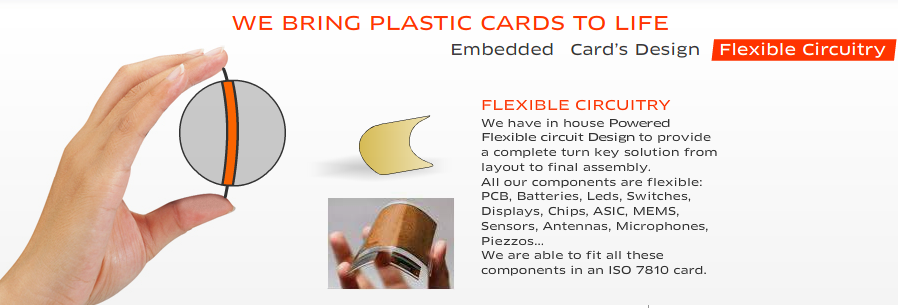
\includegraphics[width=\textwidth]{images/flx}	
	\end{figure}
\end{frame}

% ------------------------- %
\begin{frame}
\frametitle{Pr�sentation de l'entreprise (3/4)}
	\centering
	Domaines: S�curit�, sant�, jeu, marketing
	\begin{figure}
	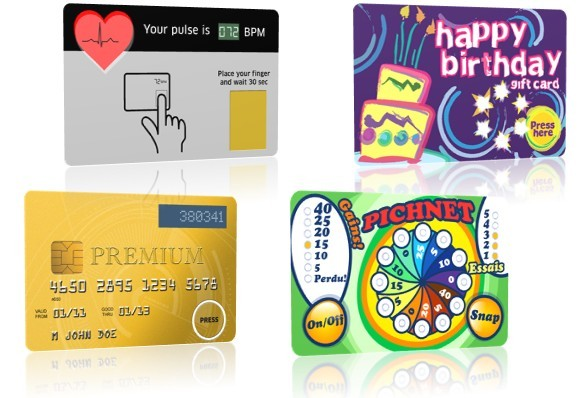
\includegraphics[scale = 0.6]{images/carte.jpg}	
	\end{figure}
\end{frame}

% ------------------------- %
\begin{frame}
\frametitle{Pr�sentation de l'entreprise (4/4)}
\framesubtitle{Projet Carte acoustique}
	\begin{figure}
	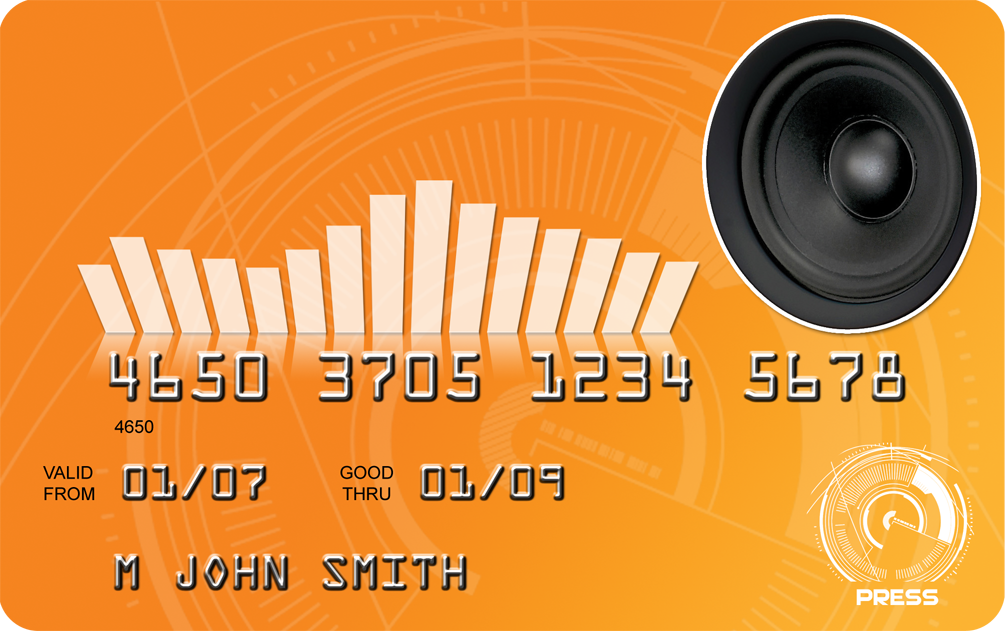
\includegraphics[scale = 0.225]{images/carteavant}	
	\caption{Face avant d'une carte acoustique}
	\end{figure}
	\begin{block}{Fonctionnalit�s g�n�rales}
La carte acoustique �met une s�quence acoustique unique � chaque pression du bouton. La carte utilise un microprocesseur pour calculer les deux OTP (One Time Password). L'�nergie utilis�e provient d'une batterie fine et flexible.
	\end{block}
\end{frame}

